Approximate convex hulls approximate the boundary of a set of points using less space than the convex hull. The points are not necessarily in 2D space, and might be in arbitrary $d$ dimensional space.
\\

Finding approximate convex hulls forms a core part of algorithms for $\epsilon$-kernels~\cite{survey} which are used in approximation algorithms~\cite{Agarwal:2004:AEM:1008731.1008736}, computer graphics~\cite{BAREQUET200191}, and data analysis~\cite{DBLP:journals/corr/AgarwalKSS17}. Non-negative matrix factorization, which is used in a wide range of applications from text mining~\cite{Berry2005} to speech denoising~\cite{schmidt-noise}, is also often transformed into a problem of finding a good approximate convex hull~\cite{Arora:2012:CNM:2213977.2213994}. We explain these connections in more detail in Chapter~\ref{chapter:related_work}.
\\

We begin by defining convex hulls, approximate convex hulls, streaming algorithms, and give an outline of our contributions.

\section{Convex Hulls}

We use a slight modification of the regular notion of convex hulls. In our definitions, a convex hull of $P$ is a subset $S$ of $P$ such that the convex closure of $S$ contains all points in $P$. In particular, $P$ is always a convex hull of $P$. Typically we are interested in an \emph{optimal} convex hull, which is a convex hull of minimal size.
\\

\begin{definition}
Given points $p_1, ..., p_n \in \mathbb{R}^n$, we say $p = \alpha_1 p_1 + ... + \alpha_n p_n$ is a \emph{convex combination} iff $\alpha_1 + ... + \alpha_n = 1$ and for all $i$, $\alpha_i \geq 0$.
\end{definition}

\begin{definition}
The \emph{convex closure} of $P$ is the set of all points $p$ that can be written as a convex combination of $P$. This is the smallest convex set containing $P$.
\end{definition}

\begin{definition}
Given a set of points $P \subseteq \mathbb{R}^n$, $S \subseteq P$ is a \emph{convex hull} of $P$ if every $p \in P$ can be represented as a convex combination of points in $S$.
\end{definition}

\begin{definition}
A convex hull is \emph{optimal} if it is of minimal size.
\end{definition}

\begin{figure}[!htb]
\centering
\begin{subfigure}[b]{.33\linewidth}
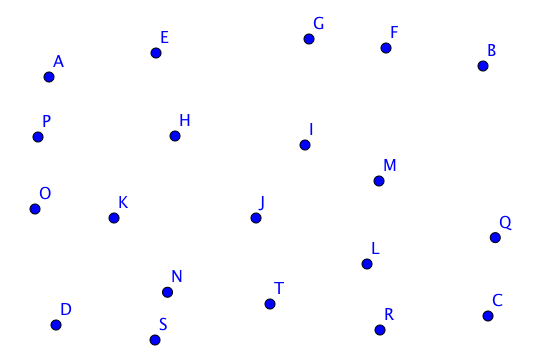
\includegraphics[width=\linewidth]{set_of_points}
\caption{Set of points}\label{fig:points}
\end{subfigure}\hspace{20 mm}
\begin{subfigure}[b]{.33\linewidth}
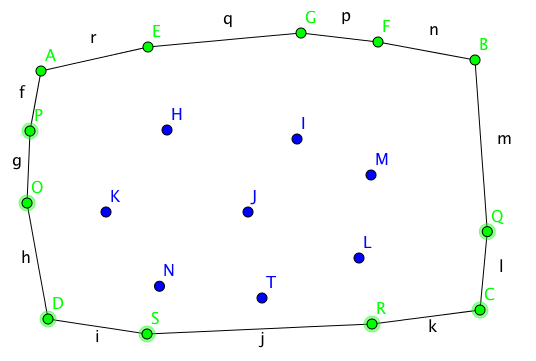
\includegraphics[width=\linewidth]{convex_hull_of_set}
\caption{Convex hull in green}\label{fig:convex_hull}
\end{subfigure}\hspace{20 mm}
\begin{subfigure}[b]{.33\linewidth}
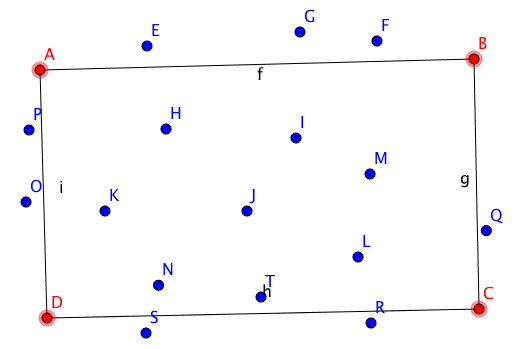
\includegraphics[width=\linewidth]{approximate_convex_hull}
\caption{Approx convex hull in red}\label{fig:approx_convex_hull}
\end{subfigure}
\caption{Convex hull and approximate convex hull of a set of points.}
\label{fig:hull_overview}
\end{figure}

Intuitively, an optimal convex hull captures the boundary of a set of points. Figure~\ref{fig:points} shows a set of points, and figure~\ref{fig:convex_hull} shows an optimal convex hull of the points. 

\section{Approximate Convex Hulls}

In many cases, we do not need to capture the boundary of a point set exactly - it suffices to have an approximation. For example, figure~\ref{fig:approx_convex_hull} highlights a smaller set of points that approximately captures the set of points. In particular, every point is either inside the approximate convex hull, or almost inside (within some distance $\epsilon$) the approximate convex hull. In these cases it is wasteful to store the entire convex hull, we can often store far fewer points and achieve a good enough approximation. We formalize these ideas with some definitions.

\begin{definition}
Given a set of points $S \subseteq \mathbb{R}^n$, we say that $p$ is an \emph{$\epsilon$-approximate convex combination} of $S$ if there exists some convex combination $q$ of points in $S$ with $|p - q|_2 \leq \epsilon$.
\end{definition}

\begin{definition}
Given a set of points $P \subseteq \mathbb{R}^n$, $S \subseteq P$ is an \emph{$\epsilon$-approximate convex hull} of $P$ if every $p \in P$ can be represented as an $\epsilon$-approximate convex combination of points in $S$. Importantly, \emph{an approximate convex hull of $P$ is made up of points in $P$}.
\end{definition}

If we don't restrict the approximate convex hull $S$ to come from the points in $P$, we can always choose 3 points that form a large triangle containing the points in $P$. However, this will typically not approximate the boundary of the original point set $P$. In Chapter~\ref{chapter:related_work} we examine some related problems where the approximate convex hull does not have to be made up of points in $P$.

\begin{figure}[!htb]
\centering
\begin{subfigure}[b]{.4\linewidth}
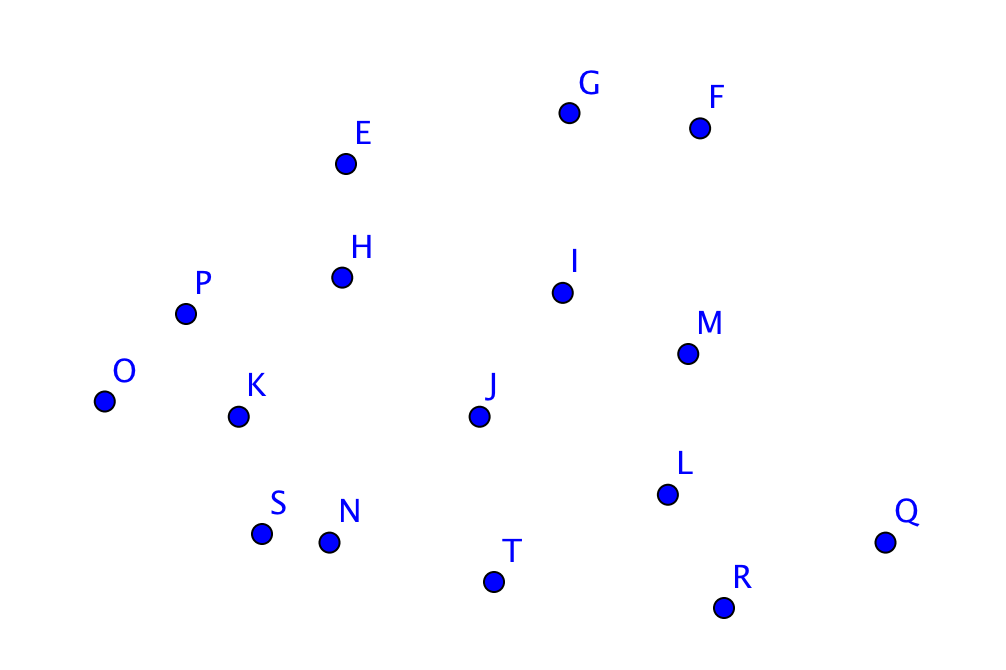
\includegraphics[width=\linewidth]{set_of_points_for_triangle}
\caption{Set of points}\label{fig:set_of_points_for_triangle}
\end{subfigure}\hspace{20 mm}
\begin{subfigure}[b]{.4\linewidth}
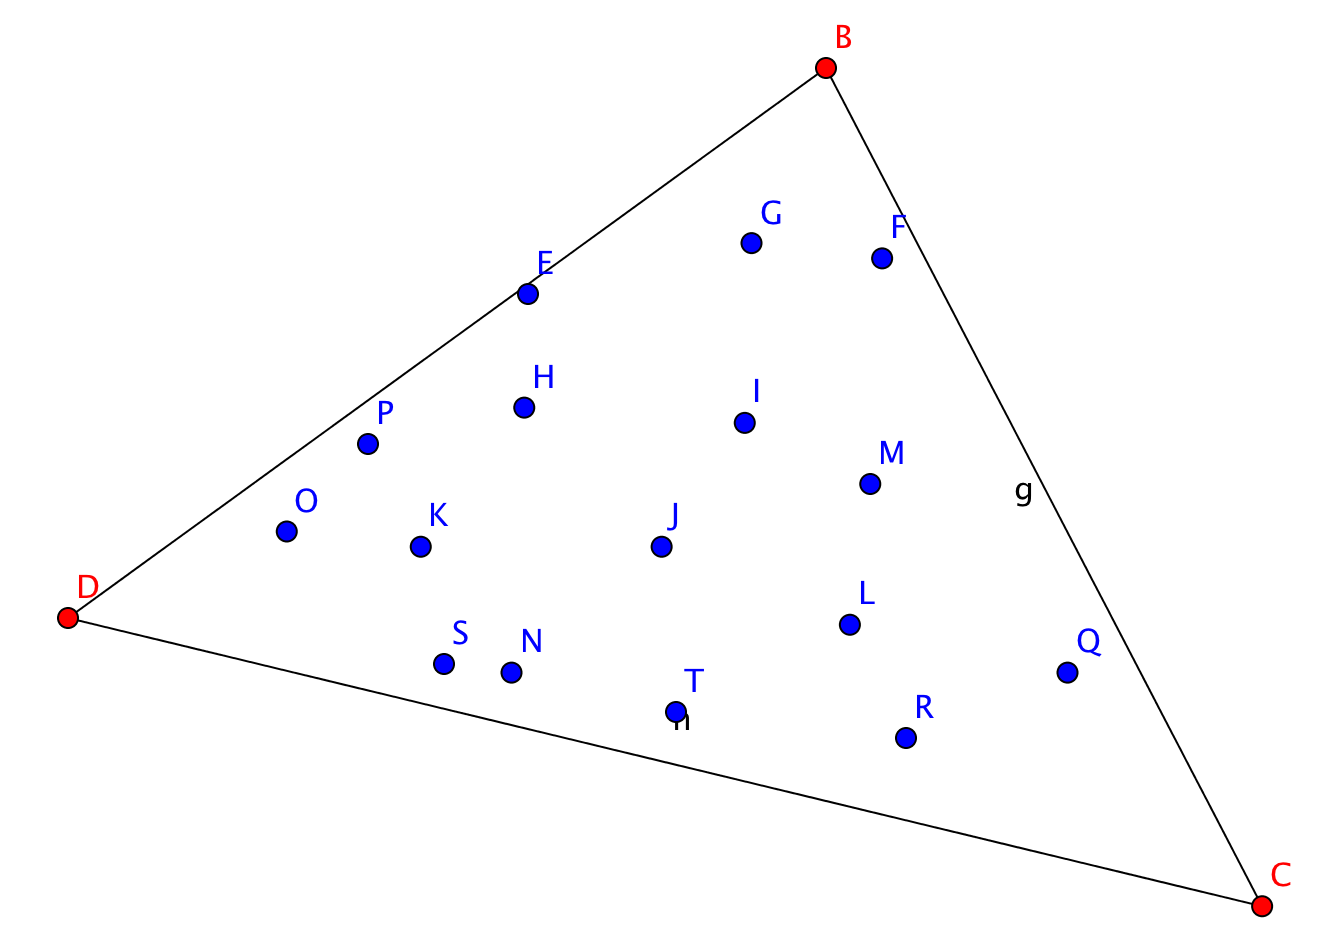
\includegraphics[width=\linewidth]{triangle_containing_set_of_points}
\caption{Triangle containing set of points}\label{fig:triangle_containing_set_of_points}
\end{subfigure}
\label{fig:triangle_containing_points}
\end{figure}

\begin{definition}
Let OPT$(P, \epsilon)$ denote the size of a (not necessarily unique) smallest $\epsilon$-approximate convex hull of $P$.
\end{definition}

\section{Batch vs Streaming}

A batch algorithm for the $\epsilon$-approximate convex hull problem takes a point set $P$, performs some sequence of operations, and outputs an $\epsilon$-approximate convex hull that is close in size to OPT$(P, \epsilon)$. In many cases, however, $P$ is too large to fit in memory.
\\

To address this, a streaming algorithm is only allowed to see each point once. After it sees the entire point set $P$, it outputs an $\epsilon$-approximate convex hull that is close in size to OPT$(P, \epsilon)$. Streaming algorithms are used in contexts where $P$ is too large to fit in memory, and are therefore assessed on the amount of memory that they use. Ideally, a streaming algorithm would use space close to OPT$(P, \epsilon)$, where $P$ is the set of points it has processed so far. Although the runtime of streaming algorithms is also important, we focus on the space complexity of streaming algorithms.
\\

We often distinguish between a set of points and a stream of points. A set of points is unordered, while a stream of points is ordered and might even contain duplicates of the same point (at different locations in the ordering).

\section{Contributions}
\label{sec:contributions}

The main aim of this thesis is to come up with good streaming algorithms for finding $\epsilon$-approximate convex hulls. We show some lower bounds to justify that this is a hard problem. In particular, we show that under a reasonable streaming model it is not possible for a streaming algorithm to be competitive with OPT (in fact, an arbtirary function of OPT) in 3D or higher. This implies that we need to relax the problem or the streaming model, or the space bound needs to include some function of $\epsilon$ or $n$ (the size of the point set).
\\

We devise and prove streaming algorithms for two relaxations of the problem. In the first relaxation, the points are on a 2D plane and come in a random order. Our algorithm maintains an initially empty point set $S$. When our algorithm sees a new point $p$, it adds $p$ to $S$ if $p$ is at least distance $\epsilon$ away from the convex closure of $S$. Additionally, our algorithm keeps removing points $p \in S$ where $p$ is contained inside the convex hull of $S \setminus \{ p \}$, that is, removing $p$ does not change the convex hull of $S$. Surprisingly, for any point stream $P$, with high probability this algorithm keeps OPT$(P, \epsilon) \log{n}$ points, where $n$ is the size of $P$.
\\

In the second relaxation, the points come in an arbitrary order in $d$-dimensional space, but we only need to be correct in ``most" directions (all but a $\delta$ fraction of directions). Our algorithm picks $O(\frac{k^2}{\delta^2}\log{\frac{k}{\delta}})$ random unit vectors, where $k = \mbox{OPT}(P, \epsilon)$. For each of these vectors $v$, we keep the point in the stream that has maximal dot product with $v$. We give a proof based on VC-dimension to show that this algorithm achieves the desired bound. For 2D we achieve an even stronger bound.
\\

Both our algorithms are simple, and we find the fact that they achieve these bounds to be surprising. These algorithms and their proofs are the core contributions of this work.
\\

Another contribution of our work is to explain some of the connections between coresets, non-negative matrix factorization, and $\epsilon$-approximate convex hulls, and their limitations. We give some experimental evidence for the connection between non-negative matrix factorization and our notion of approximate convex hulls.
\\

There has been lots of recent work on $\epsilon$-approximate convex hulls, and even streaming $\epsilon$-approximate convex hulls. However, to our knowledge, this is the first work that examines streaming algorithms for $\epsilon$-approximate convex hulls in relation to the optimal, that is, OPT$(P, \epsilon)$.
